\documentclass[a4paper,11pt]{report}
\usepackage[T1]{fontenc}
\usepackage[utf8]{inputenc}
\usepackage{lmodern}
\usepackage[english]{babel}
\usepackage{amsfonts}
\usepackage{hyperref}
\usepackage{graphicx}
\usepackage{subcaption}
\usepackage{float}

\title{Technical report from 31/01/2014 to 26/07/2014}
\author{Rafael Reggiani Manzo}

\begin{document}

\maketitle
\tableofcontents

\chapter{Previous meeting}
  \section{What was presented}
  Last time we met I've showed you my tentative on uncertainty regions segmentation for the whole \textit{corpus callosum} which produced no results despite the various forms of clustering that I tried to employ using FA, MD, TC, TV and RD values.

  \section{Next steps}
  So you've suggested to me to separate a regions where we can say for sure that there is uncertainty, for example where the fibre tracking have a curvature of 60 degrees, so we can be sure if I'm segmenting something useful or not.

\chapter{Work done}
So I separated a region of interest from the fibre tracking starting at the \textit{corpus callosum}.

, produced the FA map for this region, discretized it's values so I could finally apply the segmentation algorithm.

\section{Selecting the region of interest}
  First was applied the fibre tracking (adaptative Rung-Kutta 4) to the corpus callosum. But, instead of stopping the fibre when it has a curvature larger then 45 degrees, it was stopped for 60 degrees, producing the following image \ref{fig:fibres}.

  \begin{figure}[H]
    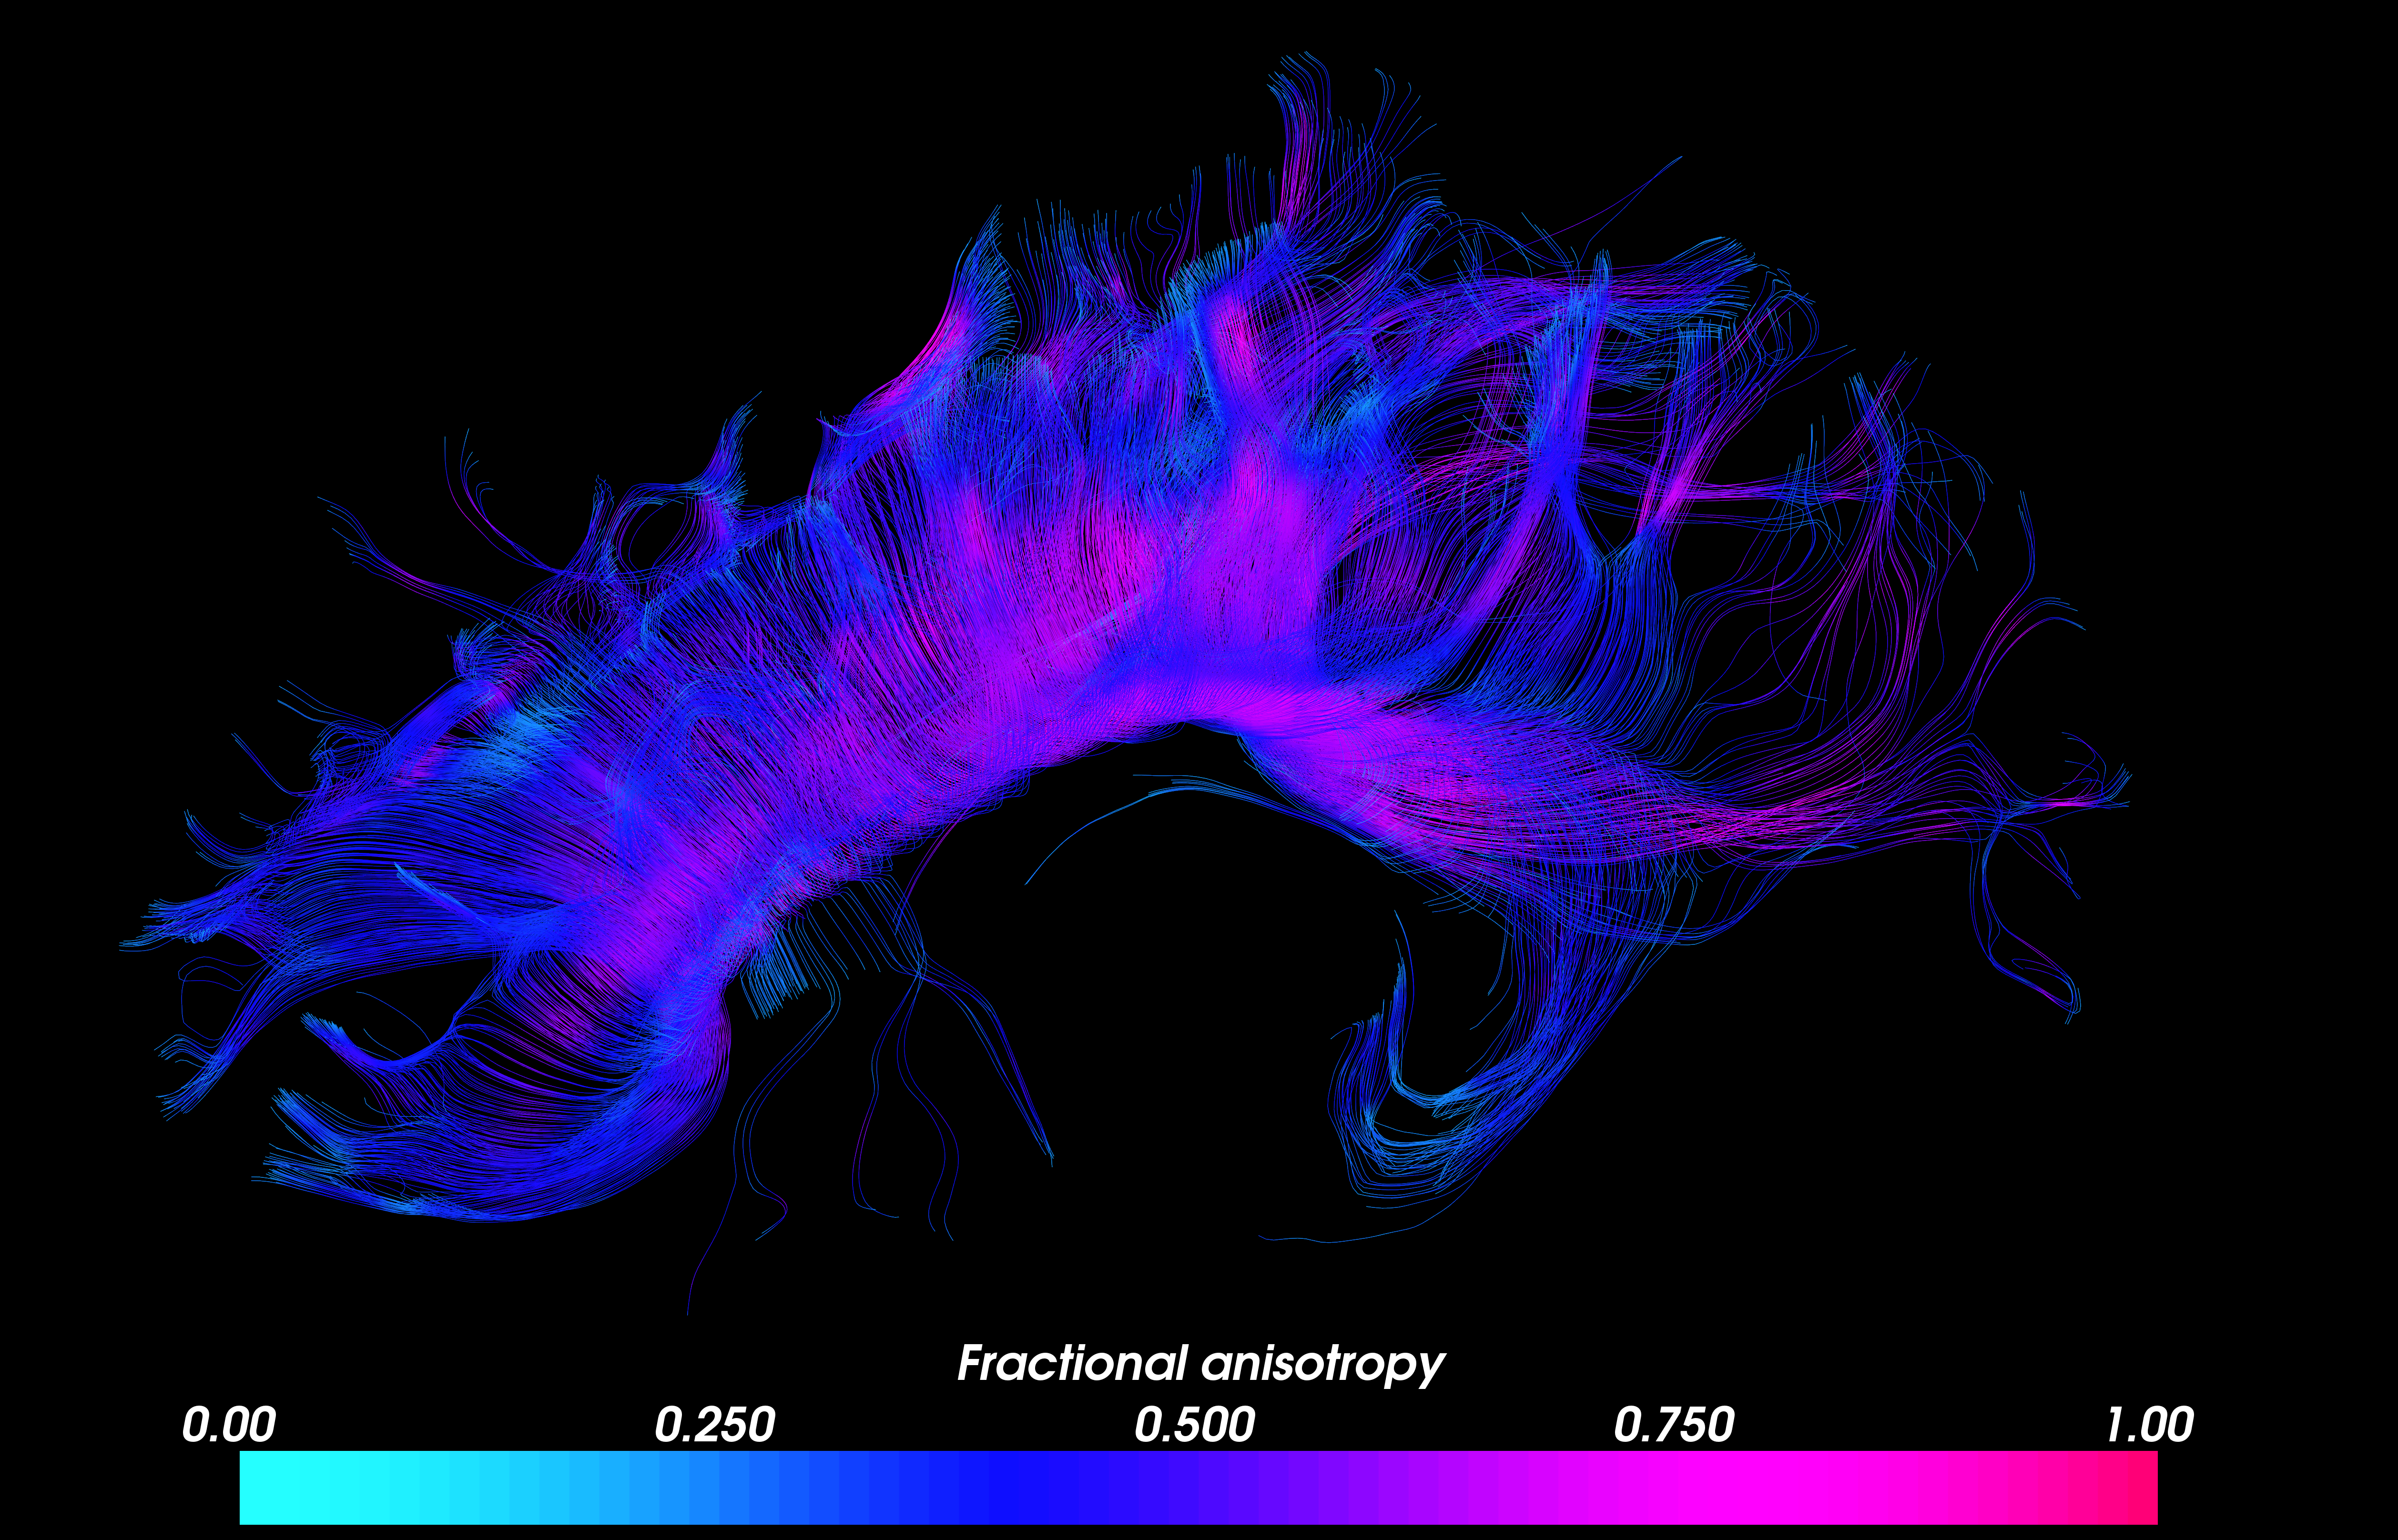
\includegraphics[width=1\linewidth]{imgs/cc-expanded-fibers.png}
    \caption{3D view of \textit{corpus callosum} with fibers tracked by the adaptive Runge-Kutta algorithm on Bio Image Suite.}
    \label{fig:fibres}
  \end{figure}

  And then exported these fibres as mask (\ref{fig:fibres-mask})

  \begin{figure}[H]
    \includegraphics[width=1\linewidth]{imgs/cc-expanded-fibers-mask.png}
    \caption{3D view of \textit{corpus callosum} with fibres tracked by the adaptive Runge-Kutta algorithm on Bio Image Suite combined with the exported mask.}
    \label{fig:fibres-mask}
  \end{figure}

  Finally cropped the mask at region where the fibre curvature is anatomically impossible (the coordinates $i$ from 83 to 96, $j$ from 65 to 88 and $k$ from 33 to 49).

  \begin{figure}[H]
    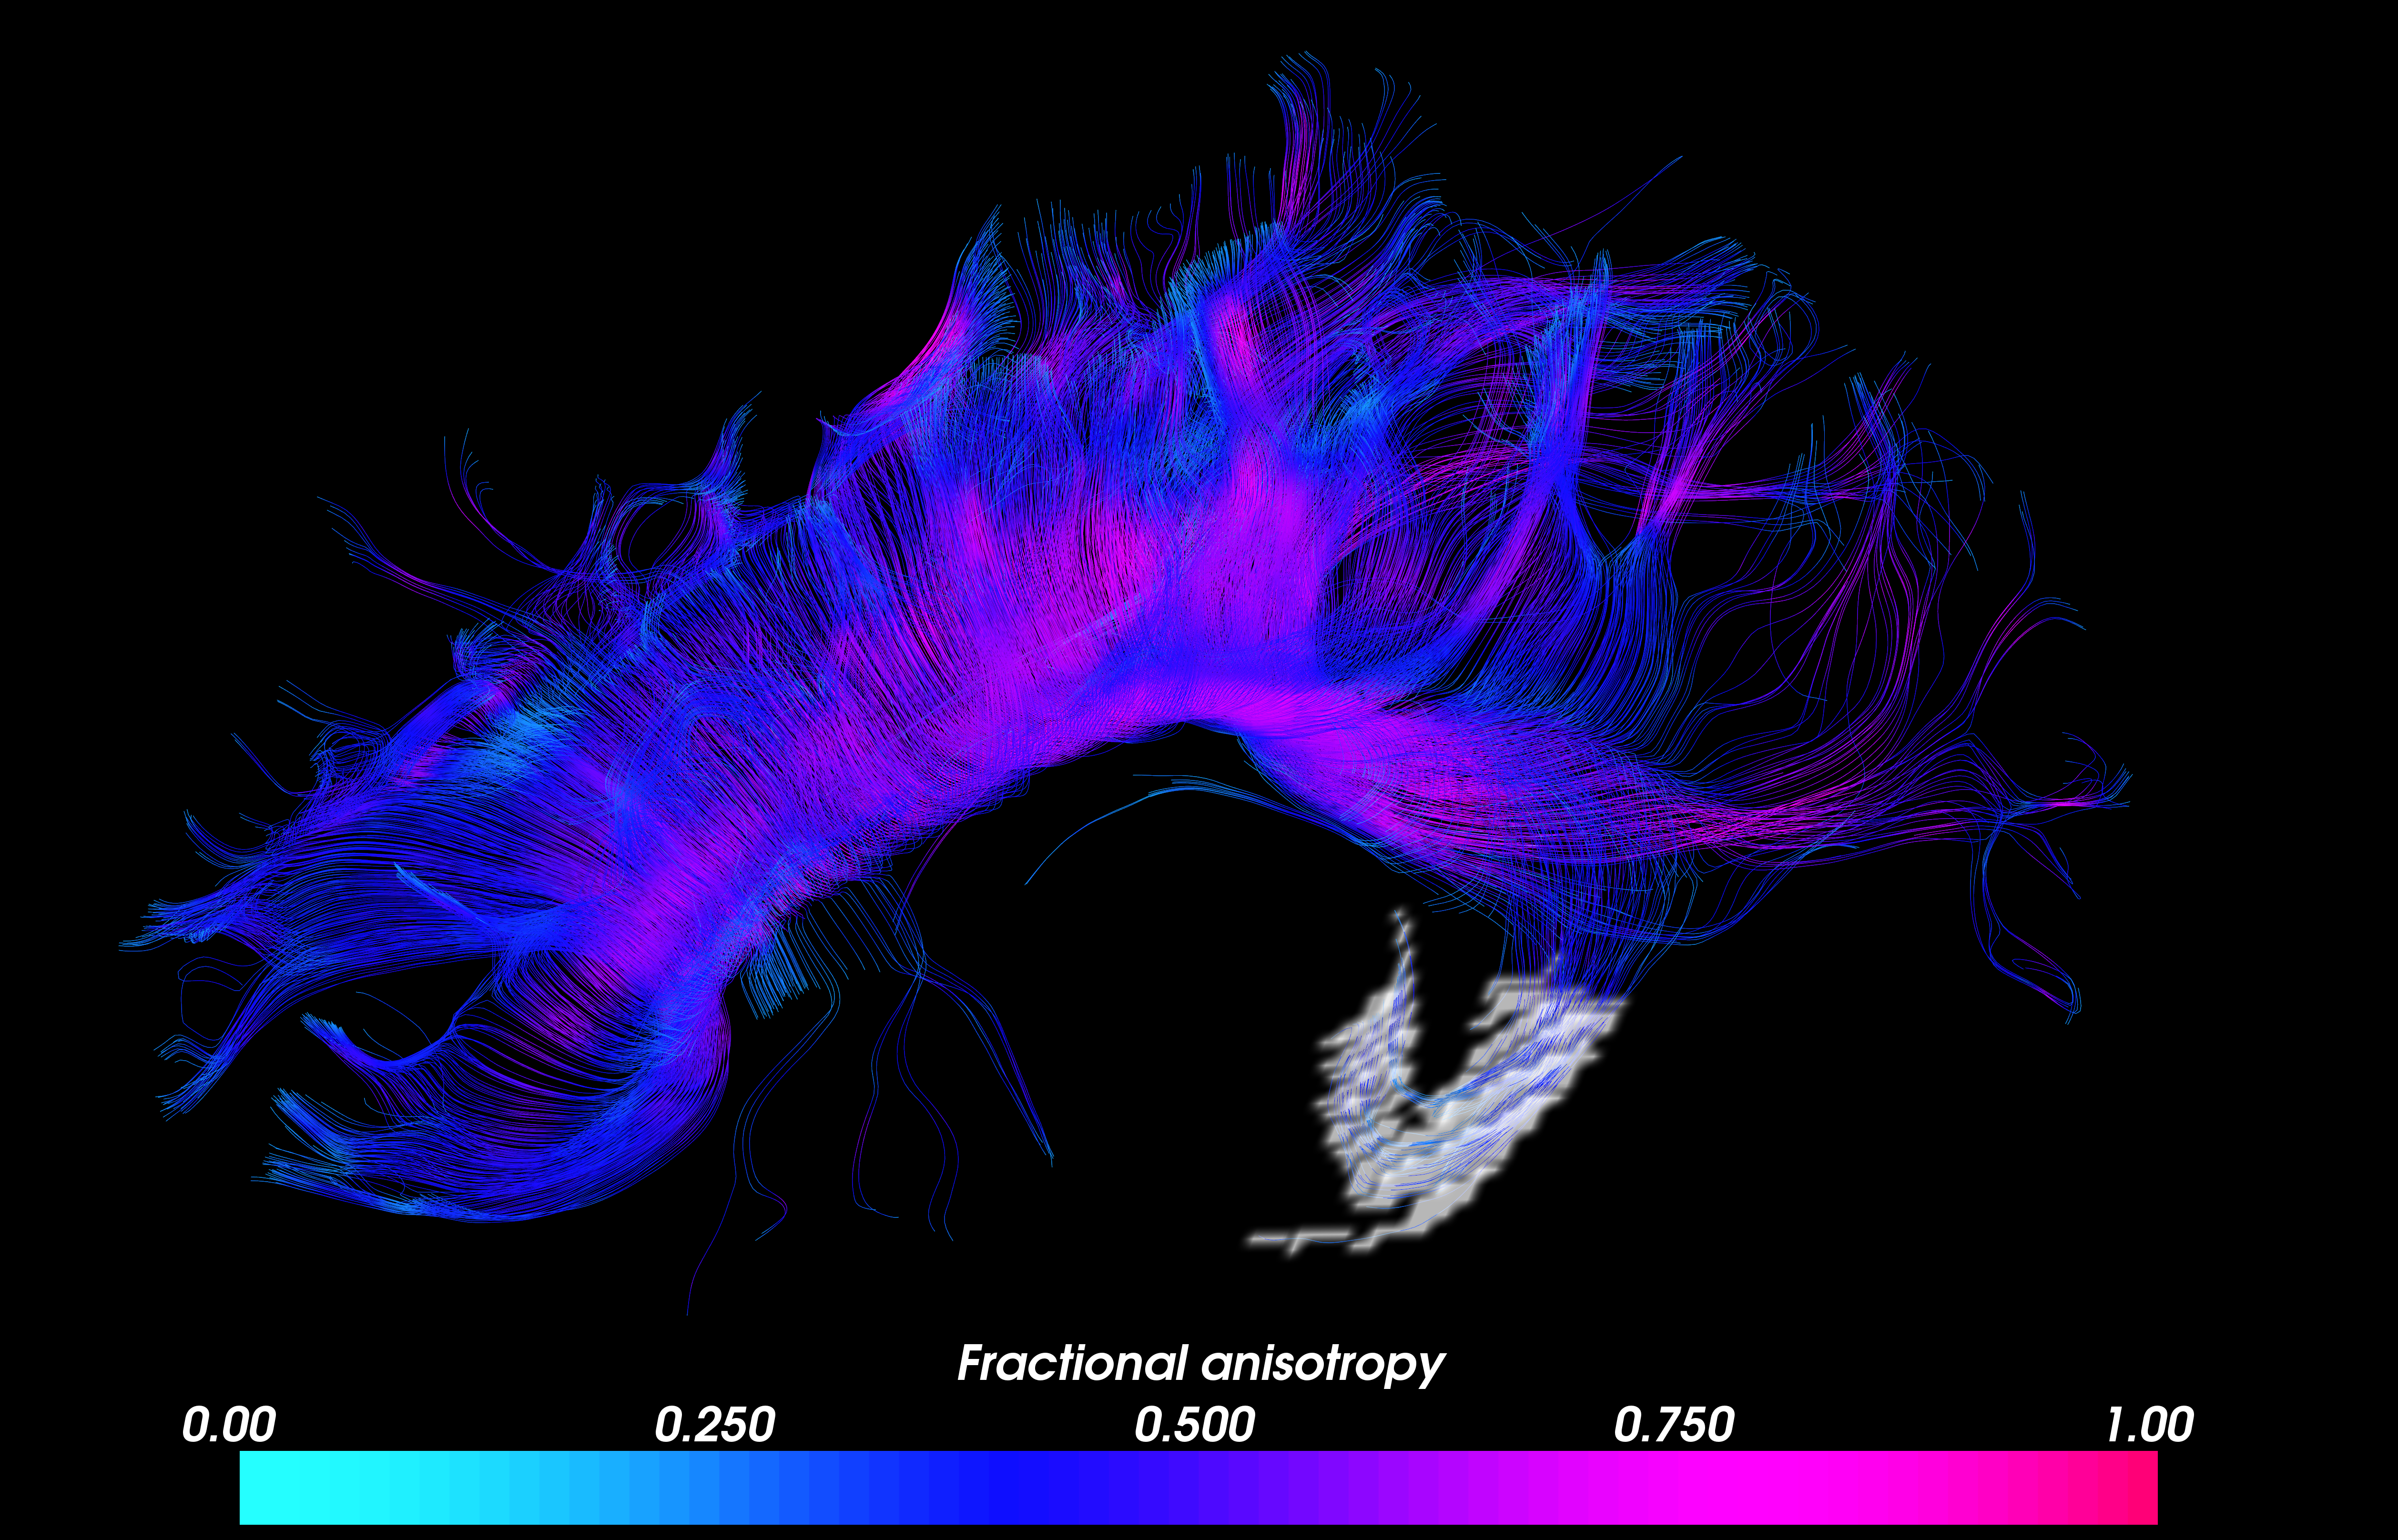
\includegraphics[width=1\linewidth]{imgs/cc-expanded-fibers-mask-croped.png}
    \caption{3D view of \textit{corpus callosum} with fibres tracked by the adaptive Runge-Kutta algorithm on Bio Image Suite combined with the exported mask cropped at region of interest.}
    \label{fig:fibres-mask-croped}
  \end{figure}

  \section{Applying clustering algorithms}

  \section{Applying a classical image segmentation algorithm}

\chapter{Next steps}

\end{document}